\documentclass[pdftex,12pt,letter]{article}
\usepackage{fancyhdr}
\usepackage{enumerate}
\usepackage{tabularx}
\usepackage{graphicx}
\usepackage{array}
\usepackage[justification=justified,singlelinecheck=false]{caption}
\usepackage{placeins}
\pagestyle{fancy}
\makeatletter
  \renewcommand\@seccntformat[1]{\csname the#1\endcsname.\quad}
\makeatother

\newcolumntype {Y}{ >{\raggedright \arraybackslash }X}
\newcommand{\HRule}{\rule{\linewidth}{0.5mm}}
\captionsetup{labelformat=empty}

\begin{document}

\begin{titlepage}
\begin{flushright}
\HRule \\[0.4cm]
{ \bfseries
{\huge Functional Test Requirements\\[1cm]}
{\Large for\\[1cm]}
{\huge CWRUtility\large\\[4cm]}
{\large Prepared by\\Jason Kuster, Stuart Long, and William Ordiway\\[1cm]
Version 1.0\\[1cm]
KOALAA Development\\[1cm]
November 12, 2012}}
\end{flushright}
\end{titlepage}
\tableofcontents{}
\begin{table}[!t]
\caption*{\bfseries Revision History}
\begin{tabularx}{\textwidth }[t]{|l|Y|Y|l|}
\hline
\bfseries Name & \bfseries Date & \bfseries Reasons for Change & \bfseries Version \\ \hline
Long & 9/22/2012 & Initial Draft & 1.0a\\
\hline
\end{tabularx}
\end{table}
\FloatBarrier
\newpage
\clearpage
\section{Main Page}
\begin{enumerate}[1.]
\item When opened, the application will display the main page.
\item From the main page, the user will be able to select any of the rest of the features of the application.
\item When the user selects a feature, the application will switch from the main page to that feature.
\item If a user "sets defaults" in either the \emph{eSuds} or \emph{NextBus} feature, the main page will accurately display the appropriate information next to the respective feature. (See the \emph{eSuds} and \emph{NextBus} for more information)
\end{enumerate}
\section{NextBus}
\section{Campus Map}
\section{eSuds}
\section{Directory}
\section{Menus}
\section{Case News}
\lfoot{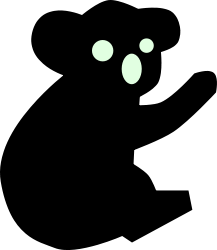
\includegraphics[height=1cm]{DarkKoala.png}}
\end{document}